\documentclass[a4paper,14pt]{extarticle}

\usepackage[a4paper,top=20mm,bottom=20mm,left=30mm,right=10mm]{geometry}
\usepackage[T1,T2A]{fontenc}
\usepackage[utf8]{inputenc}
\usepackage[russian]{babel}
\usepackage{indentfirst}
\usepackage{titlesec}
\usepackage{graphicx}
\usepackage{listings}

\renewcommand{\baselinestretch}{1.3}
\titleformat{\section}{\normalsize\bfseries}{\thesection}{1em}{}
\titleformat{\subsection}{\normalsize\bfseries}{\thesection}{1em}{}
\setlength{\parindent}{12.5mm}

\begin{document}
	
	\newpage\thispagestyle{empty}
	\begin{center}
		\MakeUppercase{
			Министерство науки и высшего образования Российской Федерации\\
			Федеральное государственное бюджетное образовательное учреждение высшего образования\\
			<<Вятский Государственный Университет>>\\
		}
		Институт математики и информационных систем\\
		Факультет автоматики и вычислительной техники\\
		Кафедра электронных вычислительных машин
	\end{center}
	\vfill
	
	\begin{center}
		Отчет по лабораторной работе №2\\
		по дисциплине\\
		<<Программирование>>\\
	\end{center}
	\vfill
	
	\noindent
	\begin{tabular}{ll}
		Выполнил студент гр. ИВТб-1301-05-00 \hspace{5mm} &
		\rule[-1mm]{25mm}{0.10mm}\,/Макаров С.А./\\
		
		Руководитель зав. кафедры ЭВМ & \rule[-1mm]{25mm}{0.10mm}\,/Долженкова М.Л./\\
	\end{tabular}
	
	\vfill
	\begin{center}
		Киров 2024
	\end{center}
	
	\newpage
	\section*{Цель}
	Цель лабораторной работы: закрепить на практике знания о программировании, использую массивы в комбинации с циклами, условными конструкциями, арифметическими операциями.
	
	\section*{Задание}
	\begin{enumerate}
		\item Задан числовой одномерный массив-кольцо, насчитывающий N элементов. Вместо каждого элемента с нулевым значением поставить сумму двух предыдущих элементов массива.
		
		\item Дан одномерный массив из N элементов. Определить, образуют ли элементы массива расположенные перед первым отрицательным числом, убывающую последовательность.
		
		\item Дан массив из N чисел, содержащий только нули и единицы. Найти номер элемента с которого начинается самая длинная последовательность единиц и количество элементов этой последовательности. Если таких последовательностей несколько, вывести номер последней из них. Если единицы в исходном массиве отсутствуют - вывести дважды 0.
		
		\item Дан массив из N целых чисел. Сформировать новый массив, состоящий из элементов исходного массив, значения которых меньше их правого соседа.
		
		\item В массиве из N целых чисел выбрать максимальное количество подряд идущих элементов, сумма которых не превышала бы целого числа K.
		
		\item В заданном одномерном массиве, состоящем из N целых чисел подсчитать количество элементов, делящихся нацело на 3, и целую часть (округление по правилам арифметики) среднего арифметического элементов с четными значениями. Поставить полученные величины на первое и последнее места в исходном массиве (увеличить массив на 2 элемента).
		
		\item В прямоугольной матрице A, имеющей N строк и M столбцов найти наименьшее значение среди средних значений для каждой строки матрицы.
		
		\item Дан массив из N целых чисел, содержащий по крайней мере два нуля. Вывести сумму чисел из данного массива, расположенных между двумя последними нулями.
		
		\item Дан массив из N вещественных чисел (N < 100). Будем называть массив пилообразным, если каждый его внутренний элемент либо больше, либо меньше обоих его соседей. Например, массив 1 5 2 4 3 7 5 - пилообразный
		
		\item Дан массив из N вещественных чисел. Если данный массив образует неубывающую последовательности , то вывести 0. В противном случае вывести номер первого числа (нумерация начинается с нуля) нарушающего закономерность.
	\end{enumerate}
	
	\newpage
	\section*{Решение}
	\subsection*{Задание 1}
	\begin{figure}[h]
		\centering
		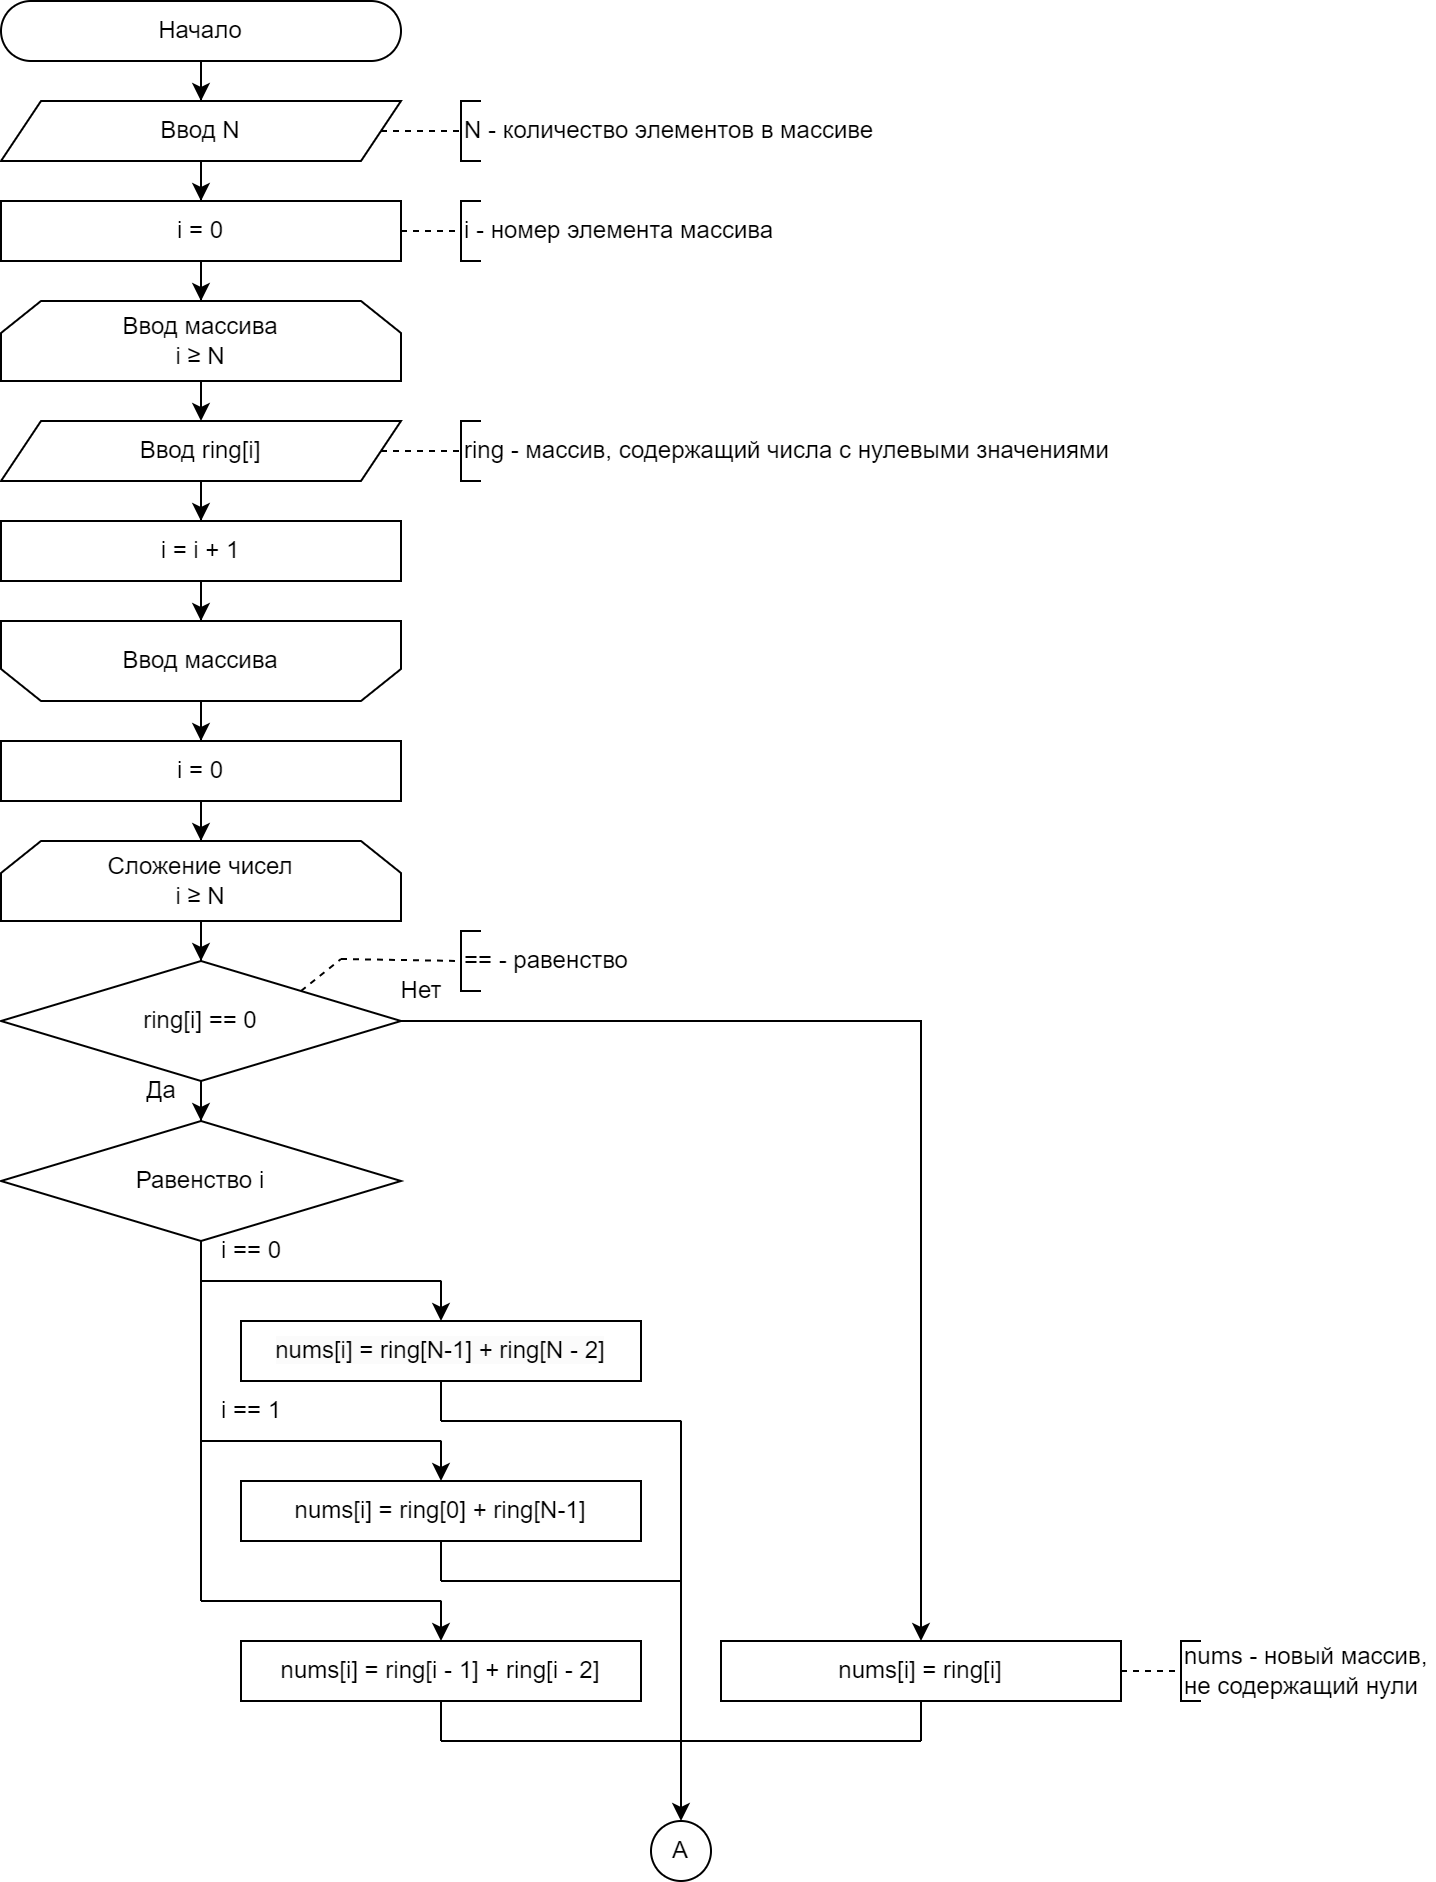
\includegraphics[width=0.89\linewidth]{schemes/s-1-1}
	\end{figure}
	\begin{center}
		Рисунок 1.1 – Схема алгоритма задания 1
	\end{center}
	\pagebreak
	\begin{figure}[h]
		\centering
		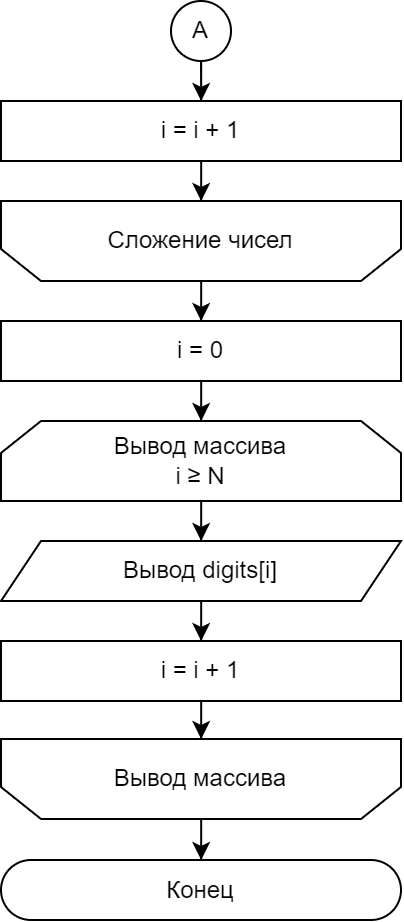
\includegraphics[width=0.25\linewidth]{schemes/s-1-2}
	\end{figure}
	\begin{center}
		Рисунок 1.2 – Продолжение схемы алгоритма задания 1
	\end{center}
	\begin{lstlisting}[tabsize=2,basicstyle=\ttfamily]
program solution13;
var N, i:integer;
var ring, nums: array[1..128] of integer;
begin
	read(N);
	for i := 1 to N do read(ring[i]);
	for i := 1 to N do
	begin
		if ring[i] = 0 then
			case i of
				1: nums[i] := ring[N] + ring[N - 1];
				2: nums[i] := ring[1] + ring[N];
				else nums[i] := ring[i - 1] + ring[i - 2];
			end
		else nums[i] := ring[i];
	end;
	for i := 1 to N do write(nums[i], ' ');
end.
	\end{lstlisting}
	
	\newpage
	\subsection*{Задание 2}
	\begin{figure}[h]
		\centering
		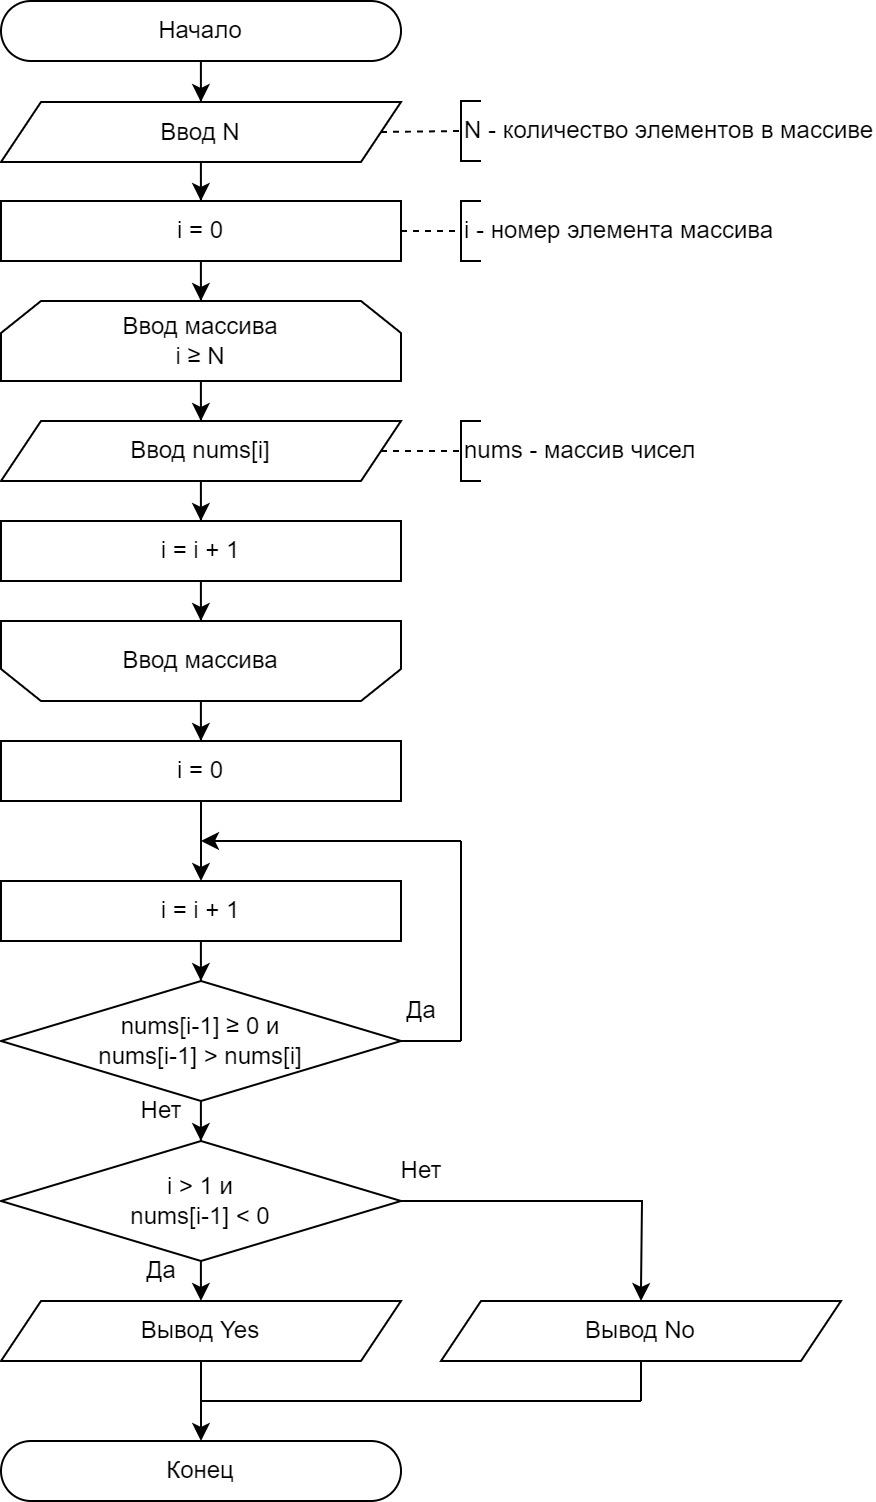
\includegraphics[width=0.5\linewidth]{schemes/s-2}
	\end{figure}
	\begin{center}
		Рисунок 2 – Схема алгоритма задания 2
	\end{center}
	\begin{lstlisting}[tabsize=2,basicstyle=\ttfamily]
#include <stdio.h>
int main() {
	int N;
	scanf("%d", &N);
	int nums[N];
	for (int i = 0; i < N; i++) {
		scanf("%d", &nums[i]);
	}
	int i = 0;
	do {
		i++;
	} while (nums[i - 1] >= 0 && nums[i - 1] > nums[i]);
	if (i > 1 && nums[i - 1] < 0) {
		printf("Yes");
	} else {
		printf("No");
	}
	return 0;
}
	\end{lstlisting}
	
	\newpage
	\subsection*{Задание 3}
	\begin{figure}[h]
		\centering
		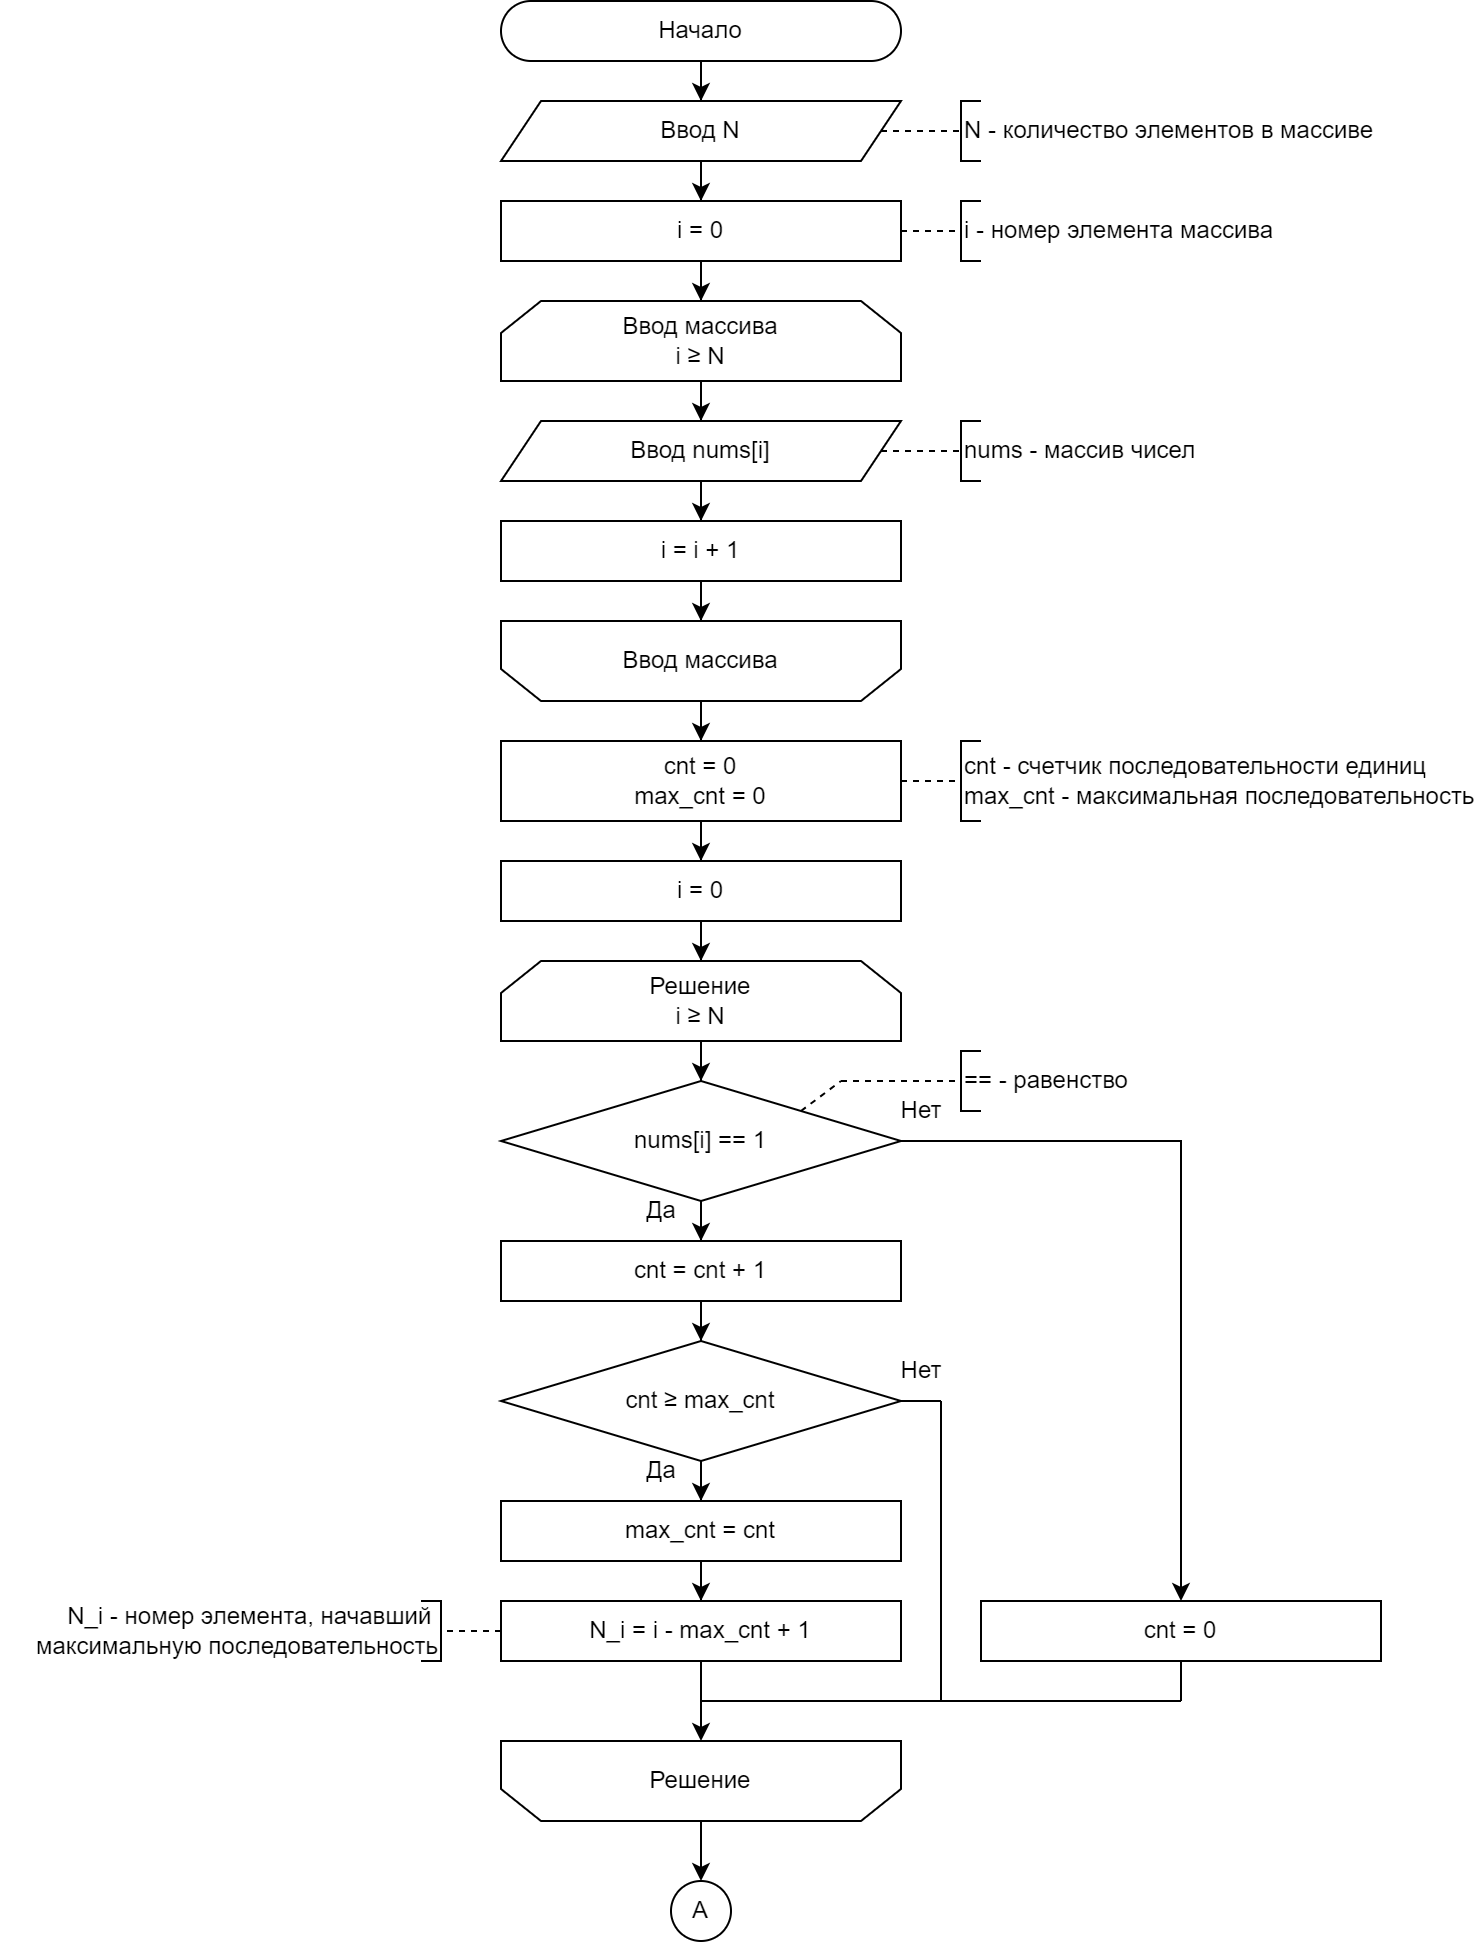
\includegraphics[width=0.89\linewidth]{schemes/s-3-1}
	\end{figure}
	\begin{center}
		Рисунок 3.1 – Схема алгоритма задания 3
	\end{center}
	\pagebreak
	\begin{figure}[h]
		\centering
		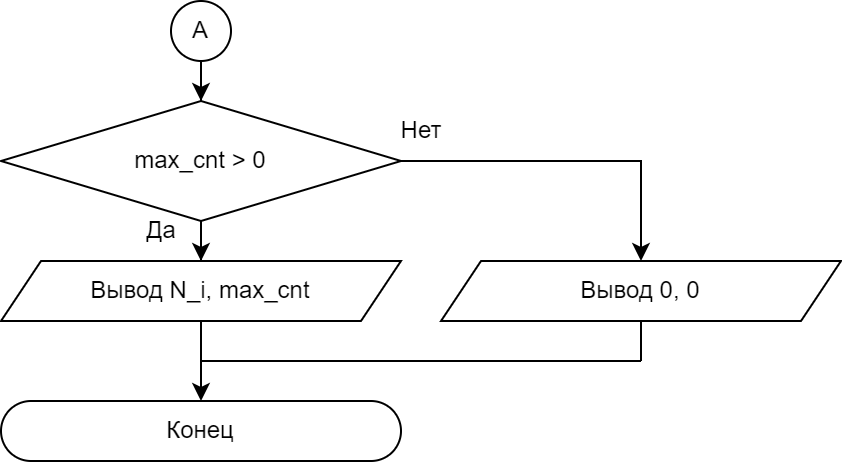
\includegraphics[width=0.55\linewidth]{schemes/s-3-2}
	\end{figure}
	\begin{center}
		Рисунок 3.2 – Продолжение схемы алгоритма задания 3
	\end{center}
	\begin{lstlisting}[tabsize=2,basicstyle=\ttfamily]
program solution15;
var N, i, cnt, max_cnt, N_i:integer;
var nums: array[1..128] of integer;
begin
	read(N);
	for i := 1 to N do read(nums[i]);
	cnt := 0;
	max_cnt := 0;
	for i := 1 to N do
	begin
		if nums[i] = 1 then
		begin
			cnt += 1;
			if cnt >= max_cnt then
			begin
				max_cnt := cnt;
				N_i := i - max_cnt;
			end;
		end
		else cnt := 0;
	end;
	if max_cnt > 0 then write(N_i, ' ', max_cnt)
	else write(0, ' ', 0);
end.
	\end{lstlisting}
	
	\newpage
	\subsection*{Задание 4}
	\begin{figure}[h]
		\centering
		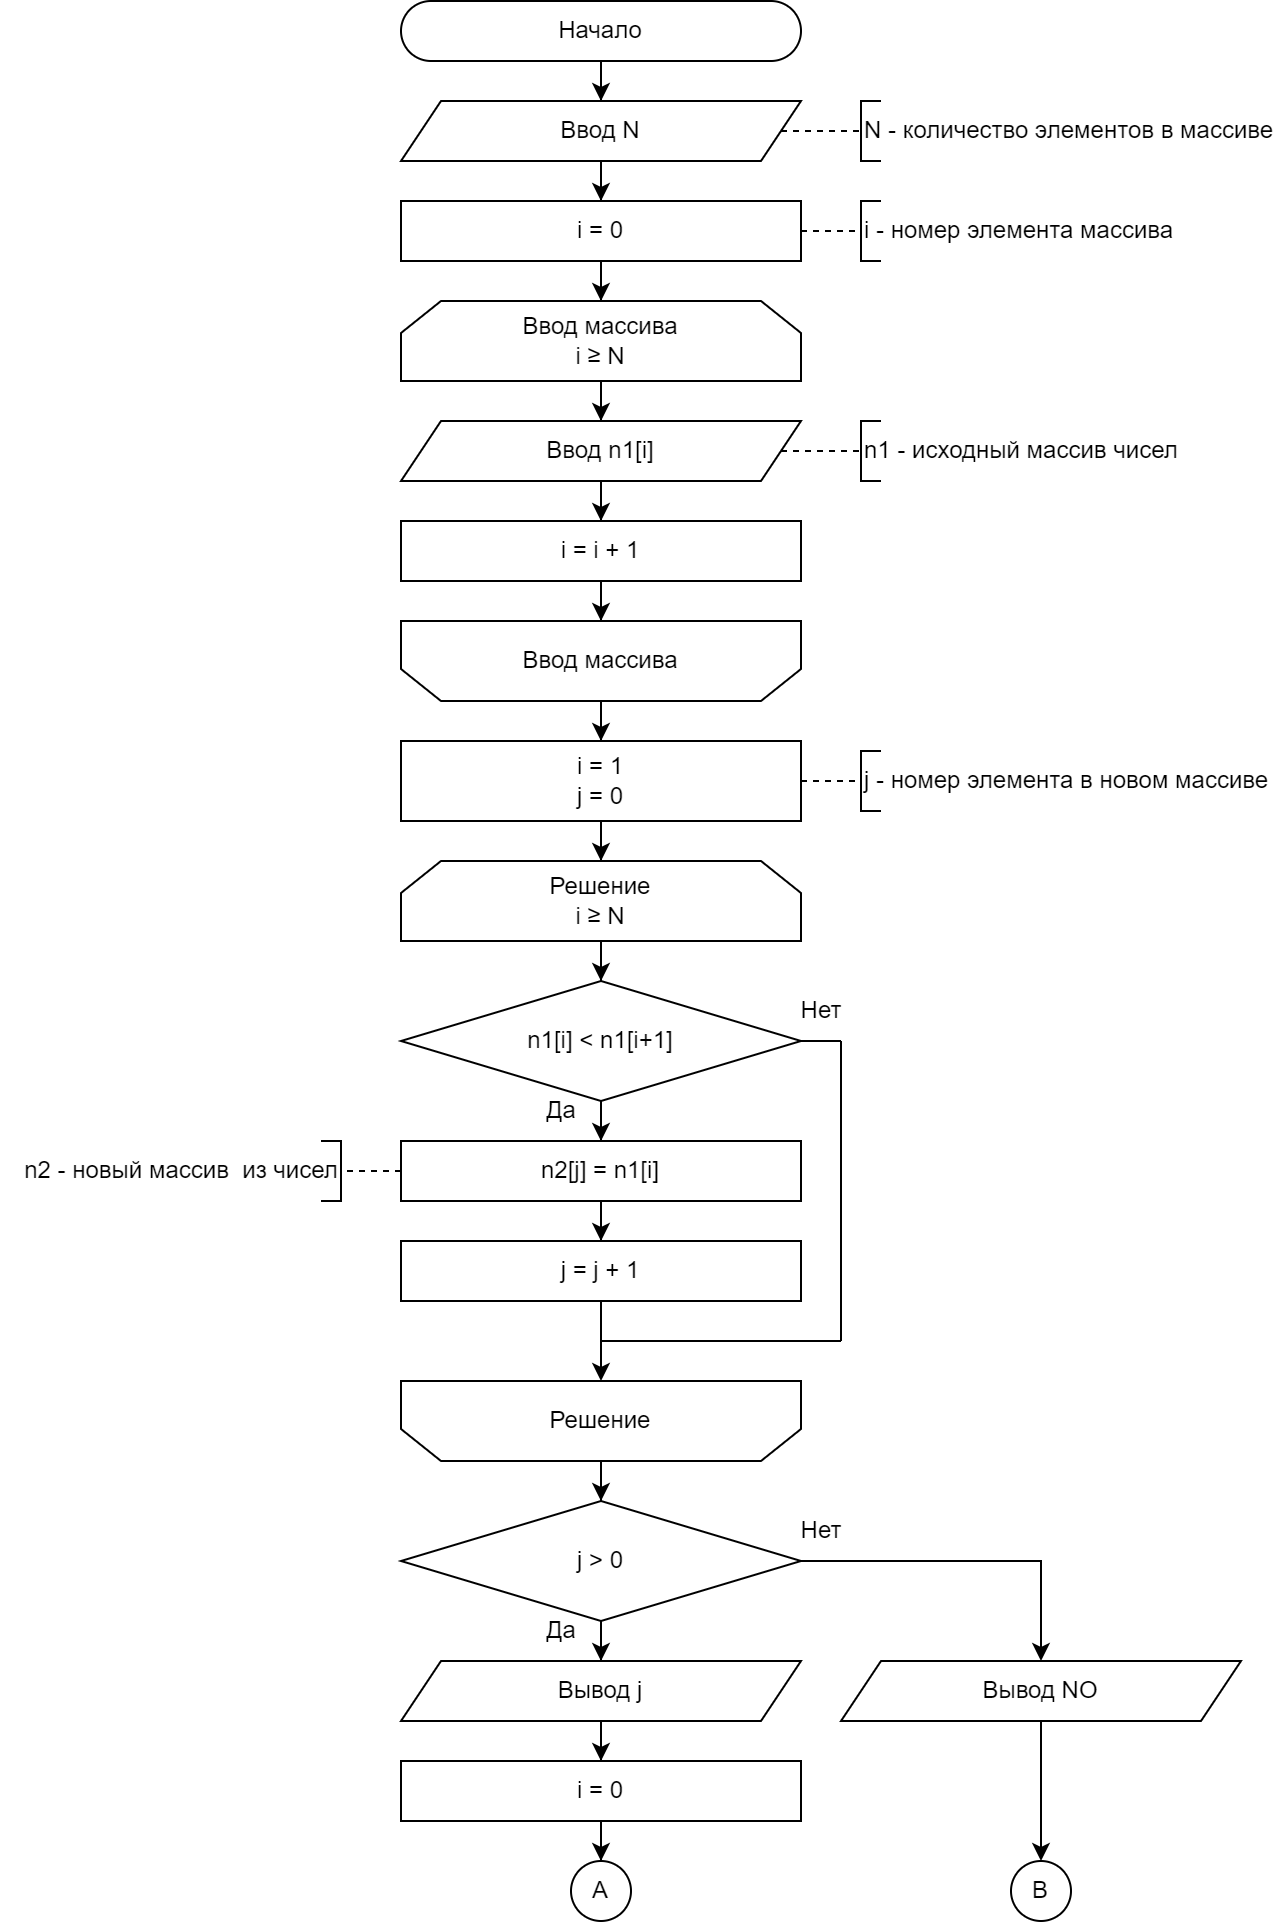
\includegraphics[width=0.78\linewidth]{schemes/s-4-1}
	\end{figure}
	\begin{center}
		Рисунок 4.1 – Схема алгоритма задания 4
	\end{center}
	\pagebreak
	\begin{figure}[h]
		\centering
		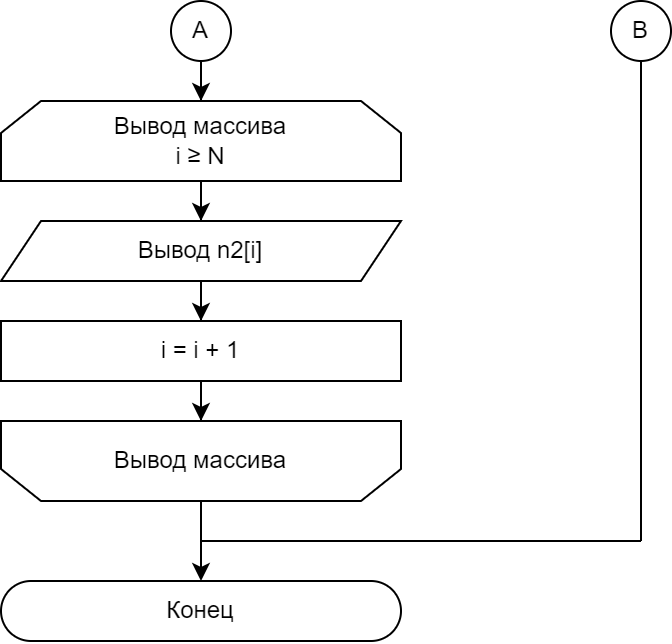
\includegraphics[width=0.45\linewidth]{schemes/s-4-2}
	\end{figure}
	\begin{center}
		Рисунок 4.2 – Продолжение схемы алгоритма задания 4
	\end{center}
	\begin{lstlisting}[tabsize=2,basicstyle=\ttfamily]
#include <stdio.h>
int main() {
	int N; scanf("%d", &N); int n1[N], n2[N];
	for (int i = 0; i < N; i++) scanf("%d", &n1[i]);
	int j = 0;
	for (int i = 1; i < N; i++) {
		if (n1[i - 1] < n1[i]) {
			n2[j] = n1[i - 1];
			j++;
		}
	}
	if (j > 0) {
		printf("%d\n", j);
		for (int i = 0; i < j; i++) {
			printf("%d ", n2[i]);
		}
	} else {
		printf("NO");
	}
	return 0;
}
	\end{lstlisting}
	
	\newpage
	\subsection*{Задание 5}
	\begin{figure}[h]
		\centering
		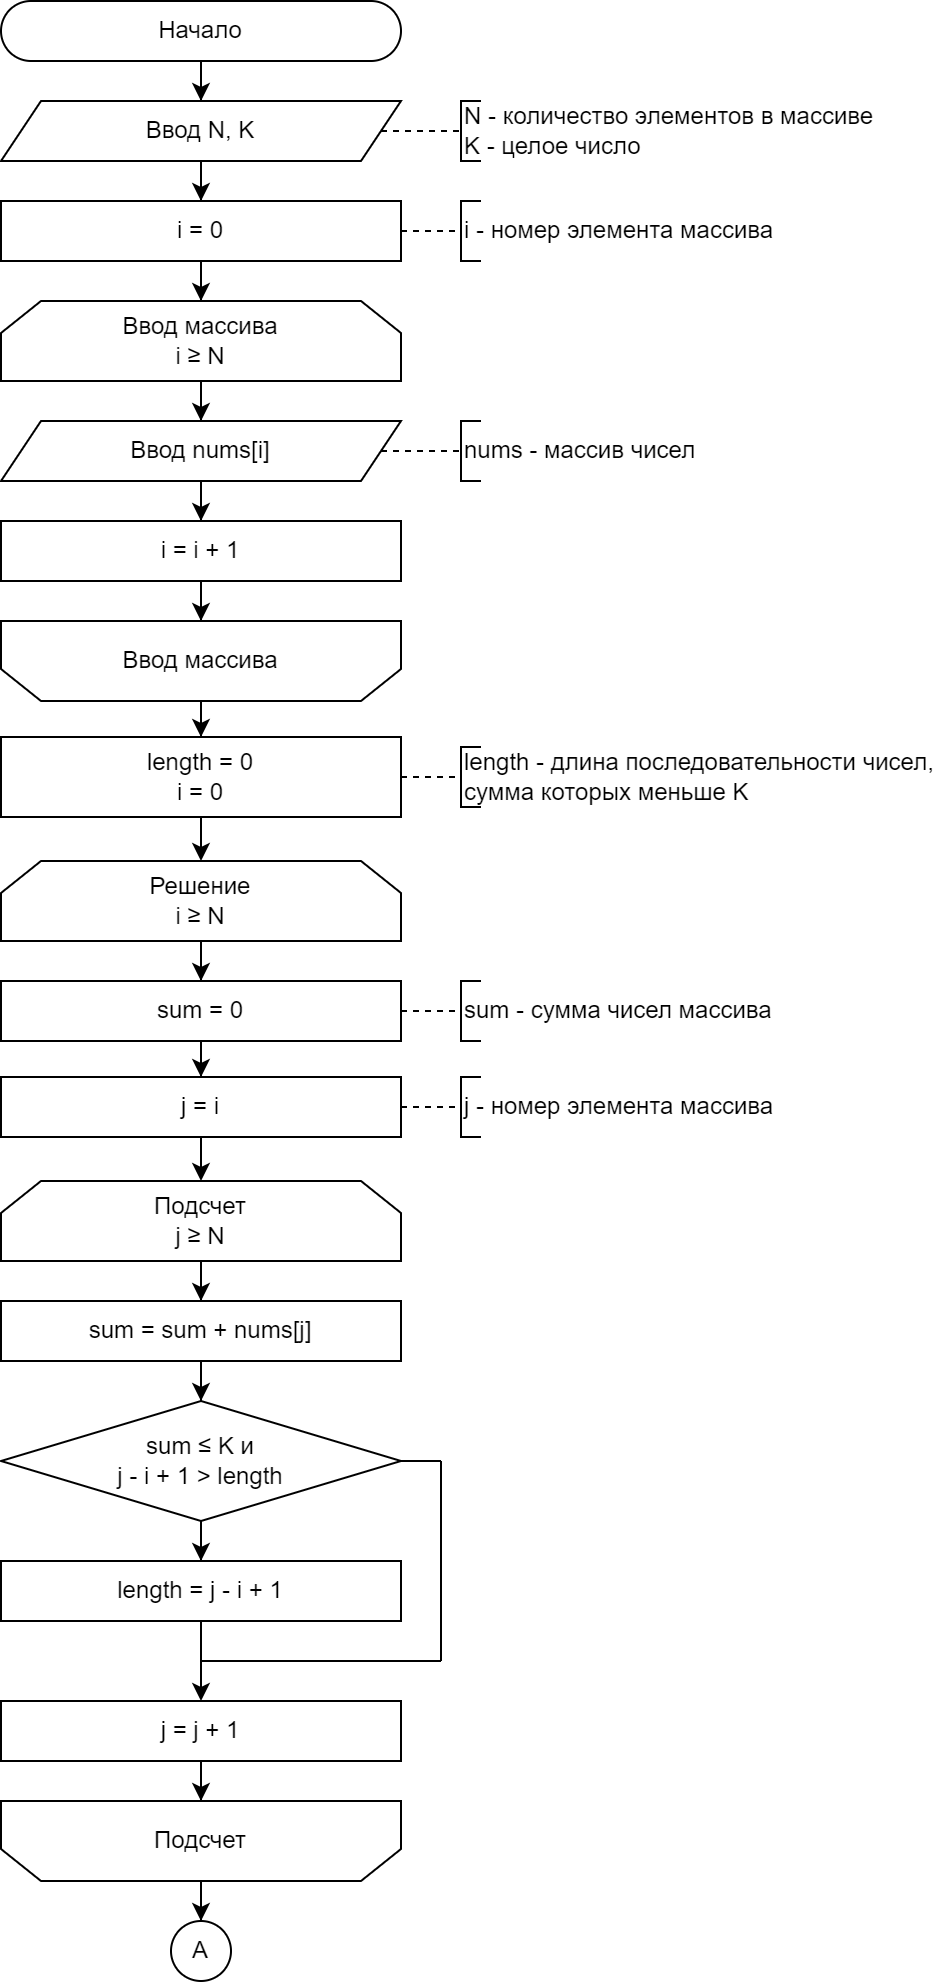
\includegraphics[width=0.55\linewidth]{schemes/s-5-1}
	\end{figure}
	\begin{center}
		Рисунок 5.1 – Схема алгоритма задания 5
	\end{center}
	\pagebreak
	\begin{figure}[h]
		\centering
		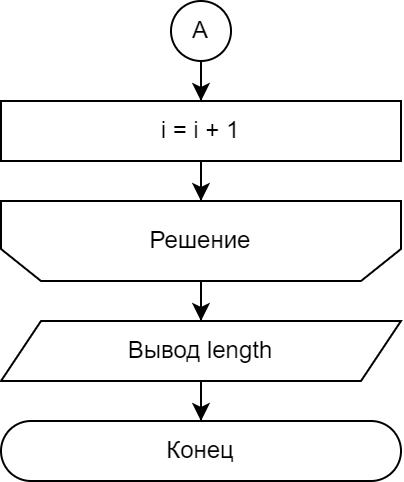
\includegraphics[width=0.25\linewidth]{schemes/s-5-2}
	\end{figure}
	\begin{center}
		Рисунок 5.2 – Продолжение схемы алгоритма задания 5
	\end{center}
	\begin{lstlisting}[tabsize=2,basicstyle=\ttfamily]
program solution17;
var N, K, i, j, length, sum:integer;
var nums: array[1..128] of integer;
begin
	read(N, K);
	for i := 1 to N do
		read(nums[i]);
	length := 0;
	for i := 1 to N do
	begin
		sum := 0;
		for j := i to N do
		begin
			sum += nums[j];
			if (sum <= K) and (j - i + 1 > length) then
				length := j - i + 1;
		end;
	end;
	write(length);
end.
	\end{lstlisting}
	
	\newpage
	\subsection*{Задание 6}
	\begin{figure}[h]
		\centering
		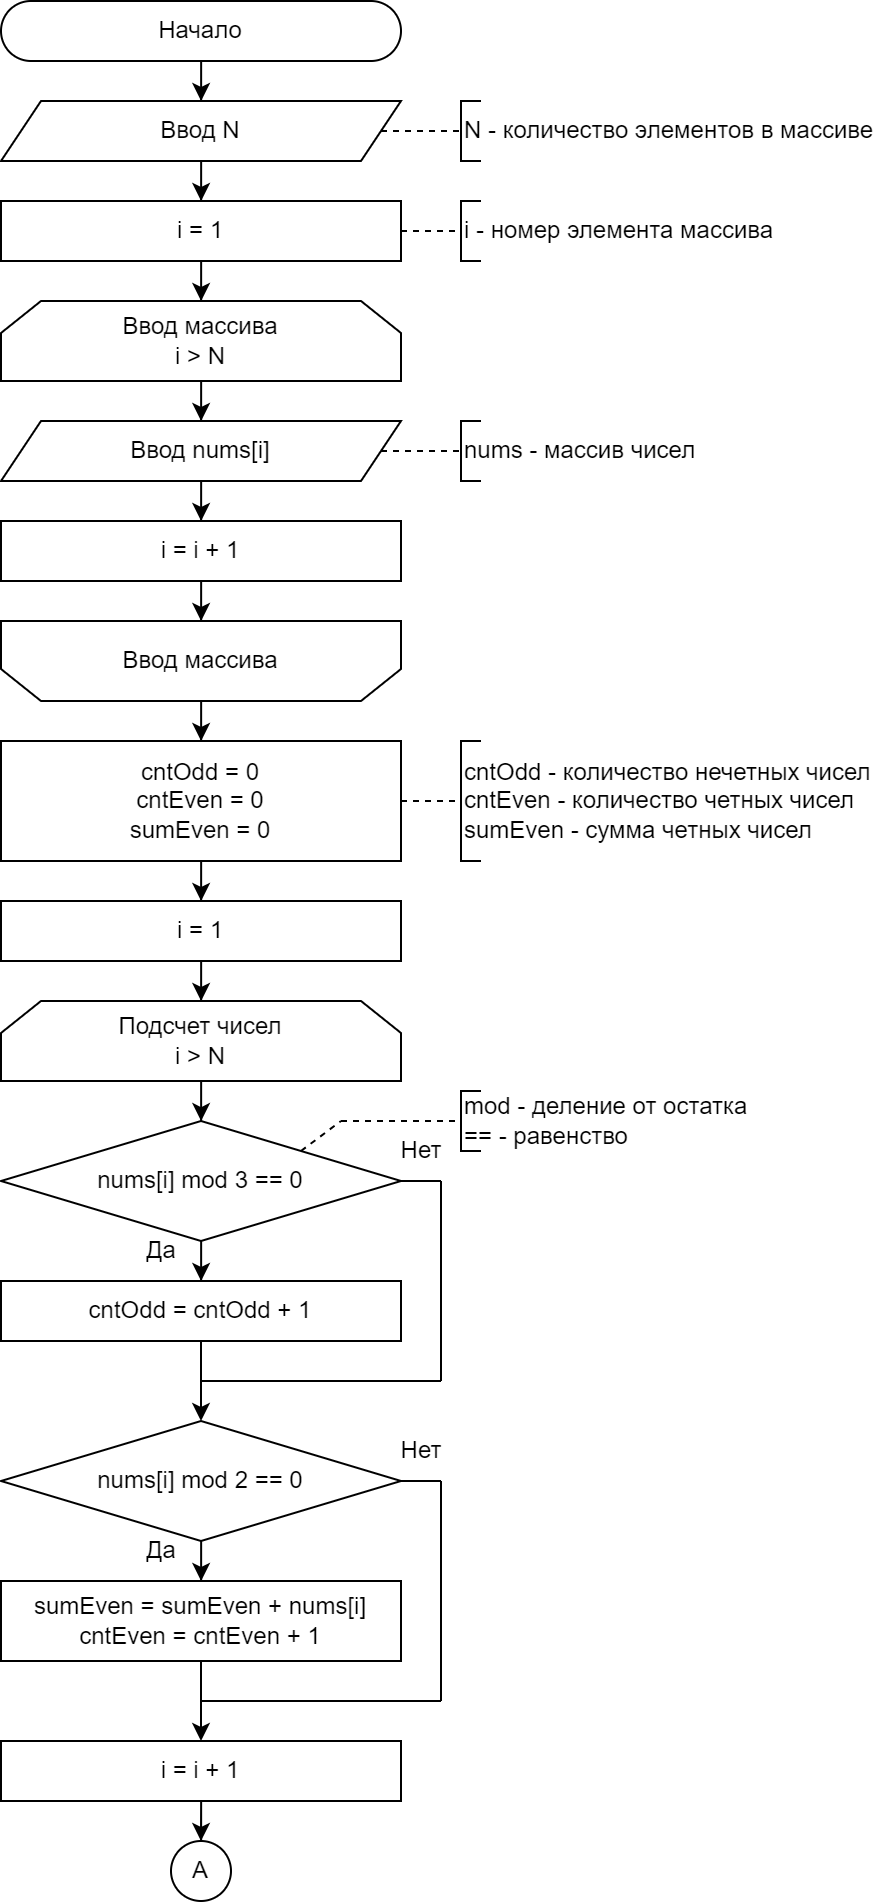
\includegraphics[width=0.54\linewidth]{schemes/s-6-1}
	\end{figure}
	\begin{center}
		Рисунок 6.1 – Схема алгоритма задания 6
	\end{center}
	\pagebreak
	\begin{figure}[h]
		\centering
		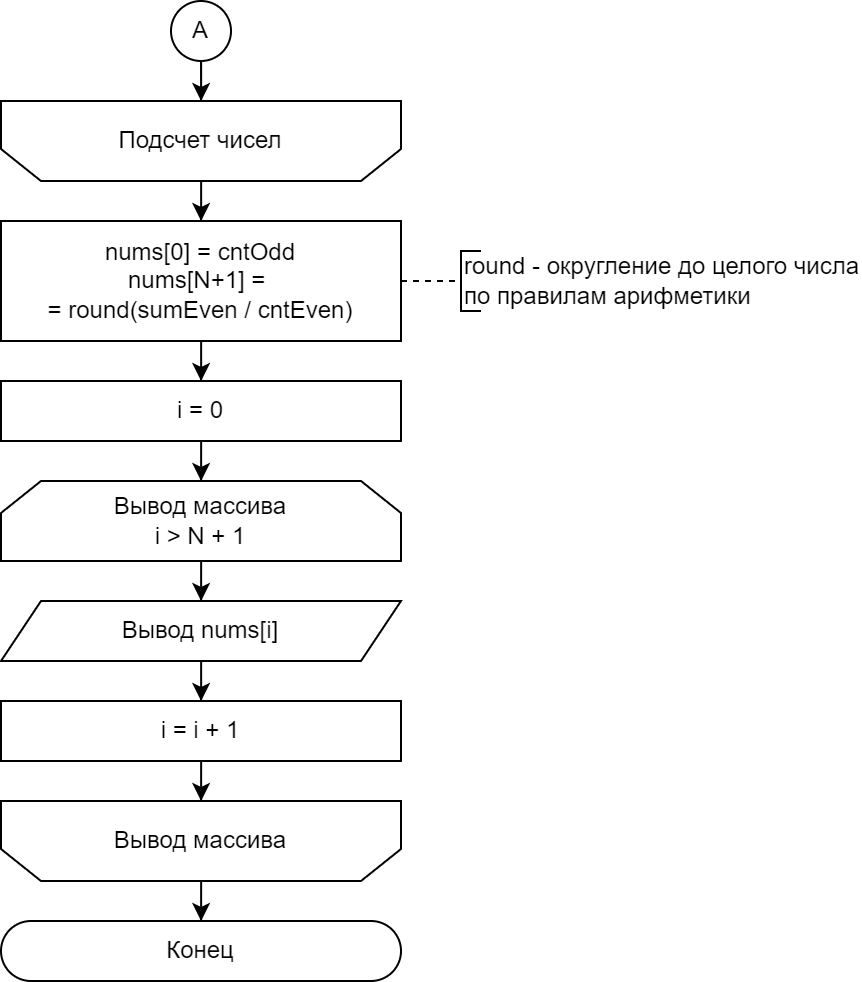
\includegraphics[width=0.55\linewidth]{schemes/s-6-2}
	\end{figure}
	\begin{center}
		Рисунок 6.2 – Продолжение схемы алгоритма задания 6
	\end{center}
	\begin{lstlisting}[tabsize=2,basicstyle=\ttfamily]
#include <stdio.h>
#include <math.h>
int main() {
	int N;
	scanf("%d", &N);
	int numbers[N + 2];
	for (int i = 1; i <= N; i++) {
		scanf("%d", &numbers[i]);
	}
	int cntOdd = 0;
	float cntEven = 0;
	float sumEven = 0;
	for (int i = 1; i <= N; i++) {
		if (numbers[i] % 3 == 0) {
			cntOdd++;
		}
		if (numbers[i] % 2 == 0) {
			sumEven += numbers[i];
			cntEven++;
		}
	}
	numbers[0] = cntOdd;
	numbers[N + 1] =  rint(sumEven / cntEven);
	for (int i = 0; i <= N + 1; i++) {
		printf ("%d ", numbers[i]);
	}
	return 0;
}
	\end{lstlisting}
	
	\newpage
	\subsection*{Задание 7}
	\begin{figure}[h]
		\centering
		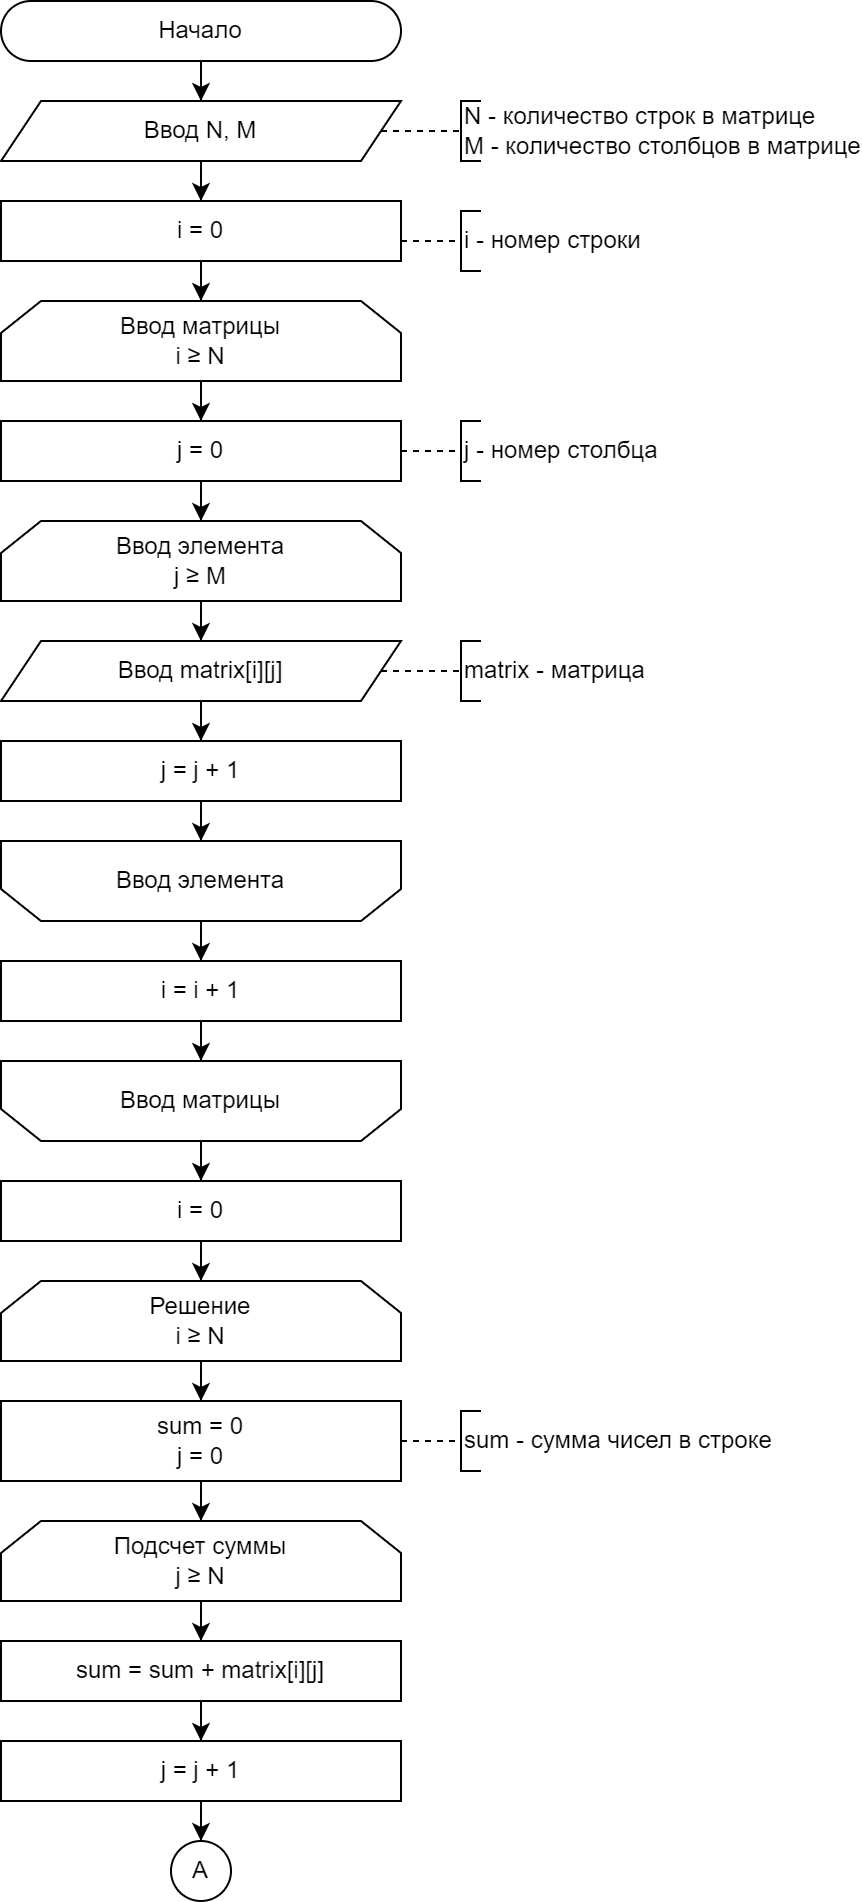
\includegraphics[width=0.53\linewidth]{schemes/s-7-1}
	\end{figure}
	\begin{center}
		Рисунок 7.1 – Схема алгоритма задания 7
	\end{center}
	\pagebreak
	\begin{figure}[h]
		\centering
		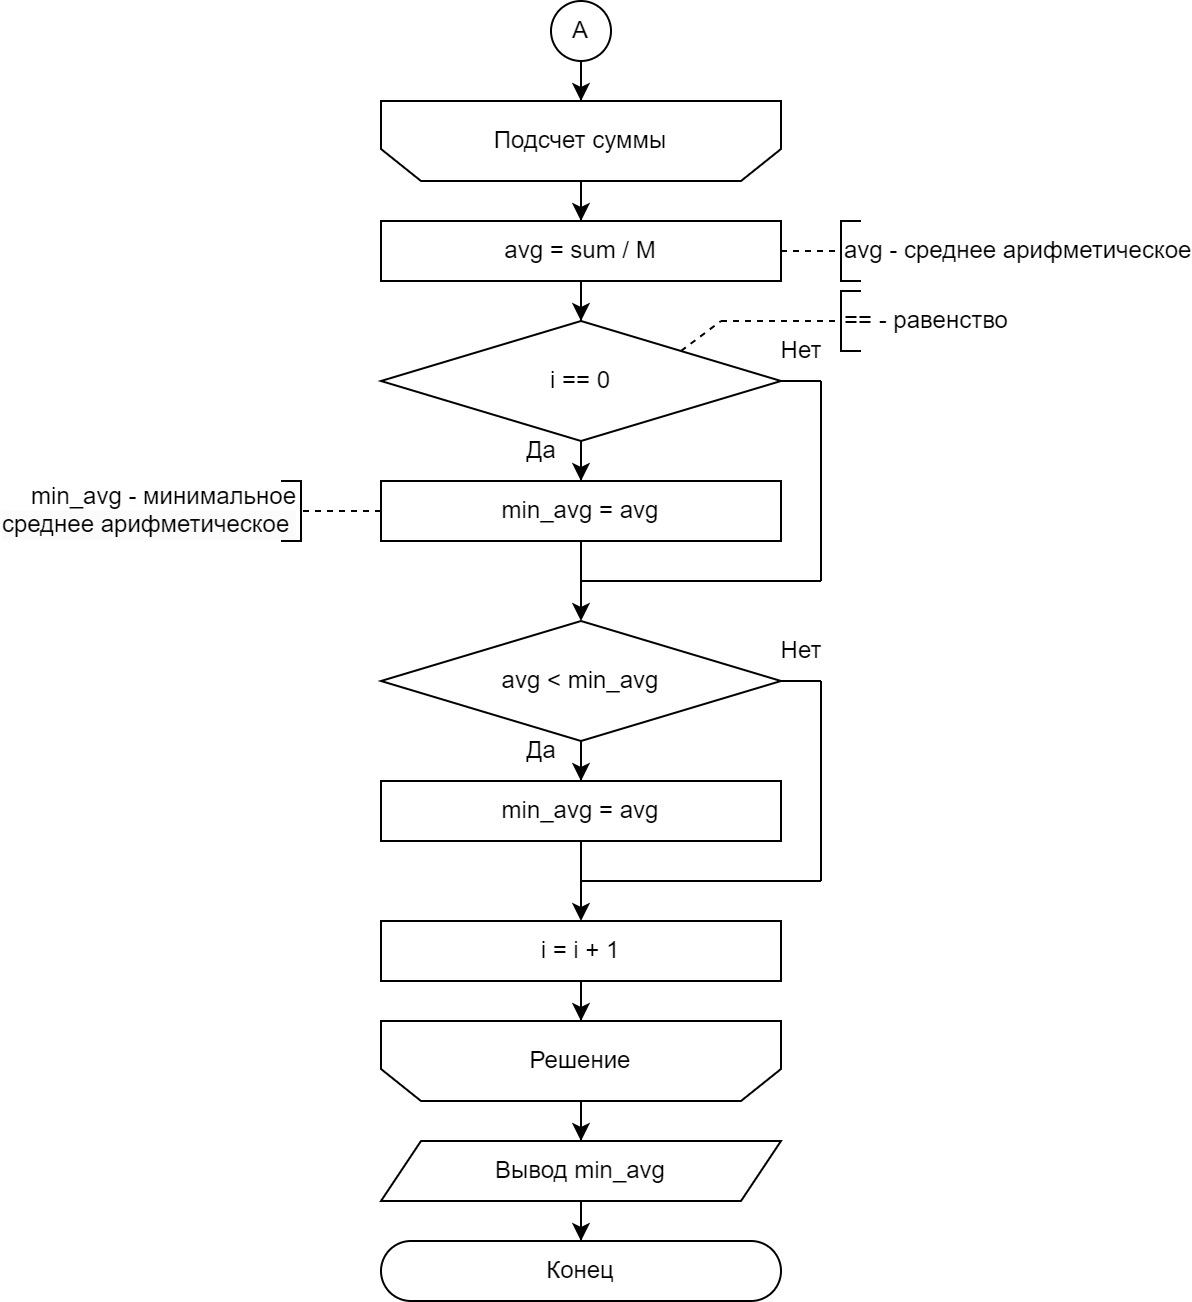
\includegraphics[width=0.8\linewidth]{schemes/s-7-2}
	\end{figure}
	\begin{center}
		Рисунок 7.2 – Продолжение схемы алгоритма задания 7
	\end{center}
	\begin{lstlisting}[tabsize=2,basicstyle=\ttfamily]
program solution19;
var N, M, i, j, sum:integer;
var avg, min_avg:real;
var matrix: array[1..16, 1..16] of integer;
begin
	read(N, M);
	for i := 1 to N do
	begin
		for j := 1 to M do
			read(matrix[i][j]);
	end;
	for i := 1 to N do
	begin
		sum := 0;
		for j := 1 to M do
			sum += matrix[i][j];
		avg := sum / M;
		if i = 1 then
			min_avg := avg;
		if avg < min_avg then
			min_avg := avg;
	end;
	write(min_avg:0:2);
end.
	\end{lstlisting}
	
	\newpage
	\subsection*{Задание 8}
	\begin{figure}[h]
		\centering
		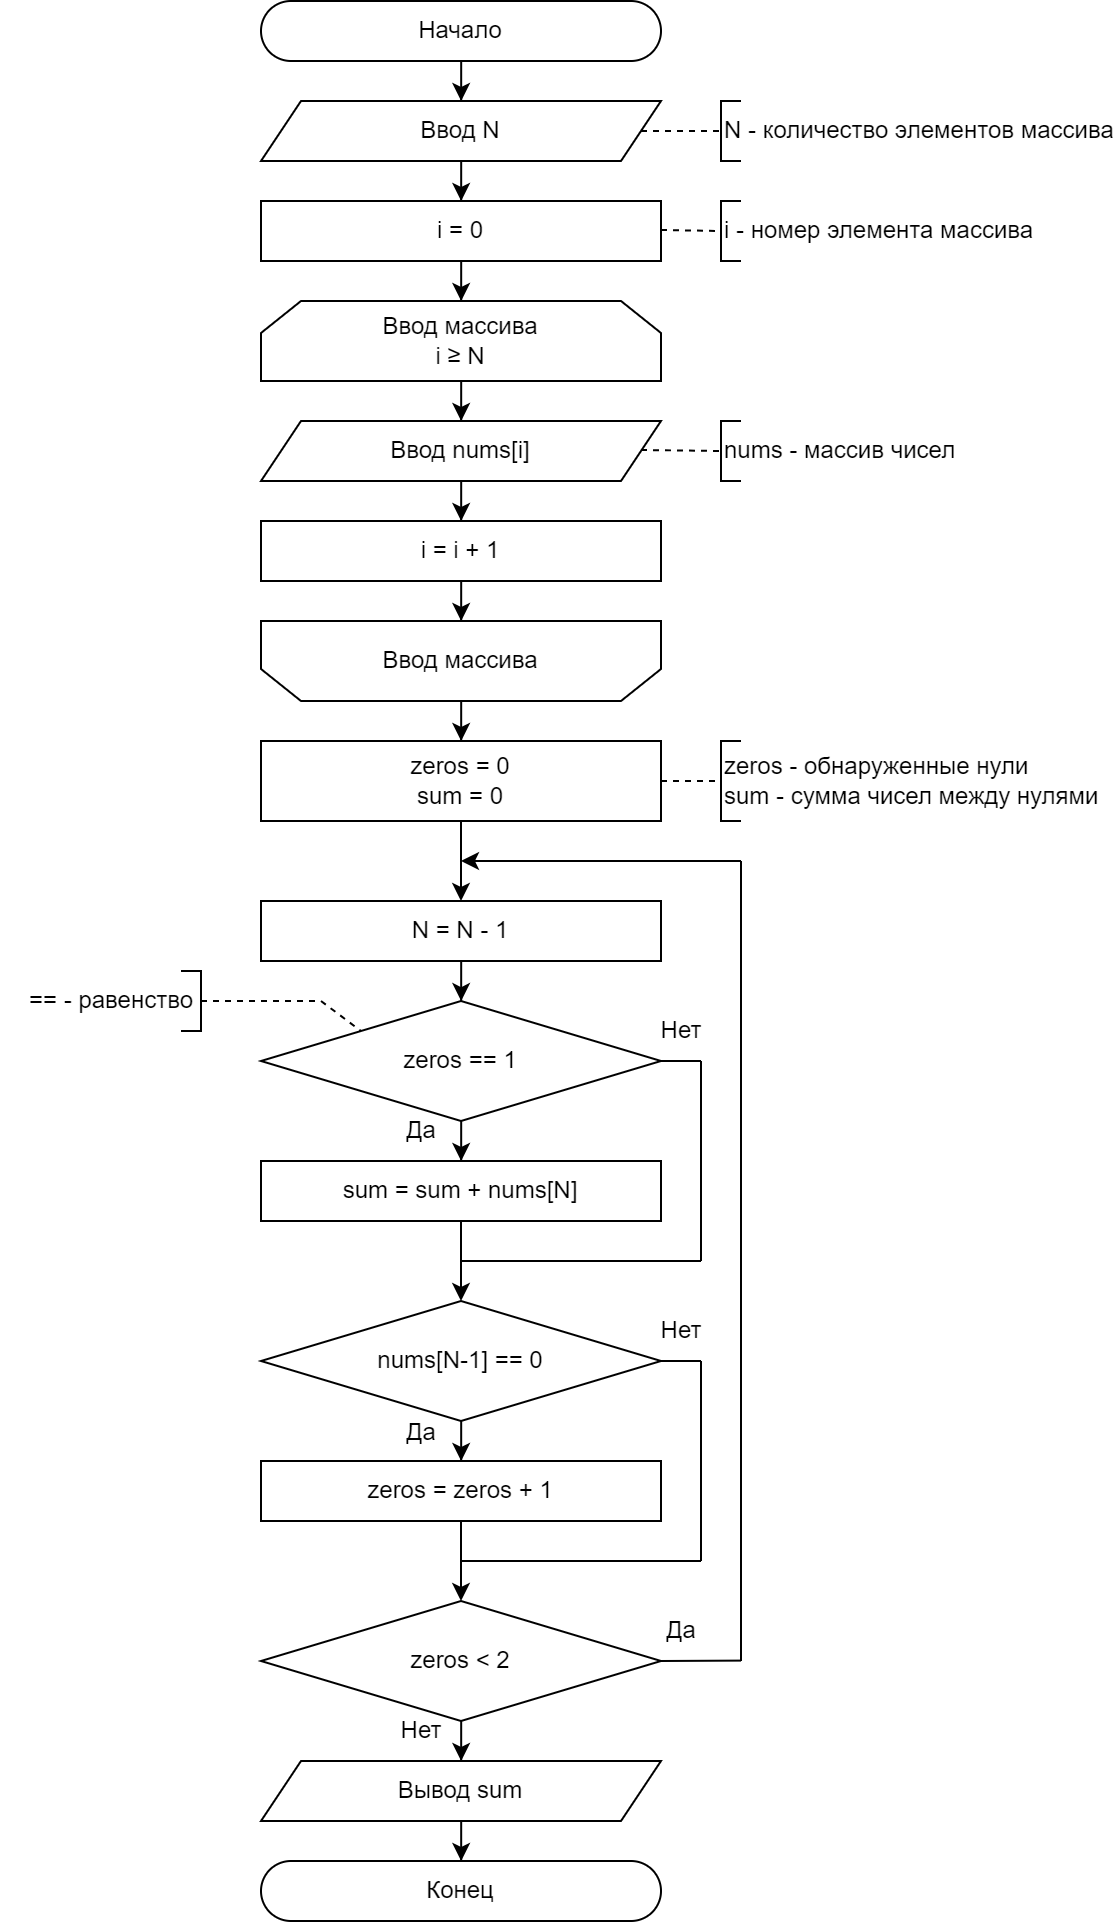
\includegraphics[width=0.68\linewidth]{schemes/s-8}
	\end{figure}
	\begin{center}
		Рисунок 8 – Схема алгоритма задания 8
	\end{center}
	\pagebreak
	\begin{lstlisting}[tabsize=2,basicstyle=\ttfamily]
#include <stdio.h>
int main() {
	int N;
	scanf("%d", &N);
	int nums[N];
	for (int i = 0; i < N; i++) {
		scanf("%d", &nums[i]);
	}
	int zeros = 0;
	int sum = 0;
	do {
		N--;
		if (nums[N] == 0) {
			zeros++;
		}
		if (zeros == 1) {
			sum += nums[N];
		}
	} while (zeros < 2);
	printf("%d", sum);
	return 0;
}
	\end{lstlisting}
	
	\newpage
	\subsection*{Задание 9}
	\begin{figure}[h]
		\centering
		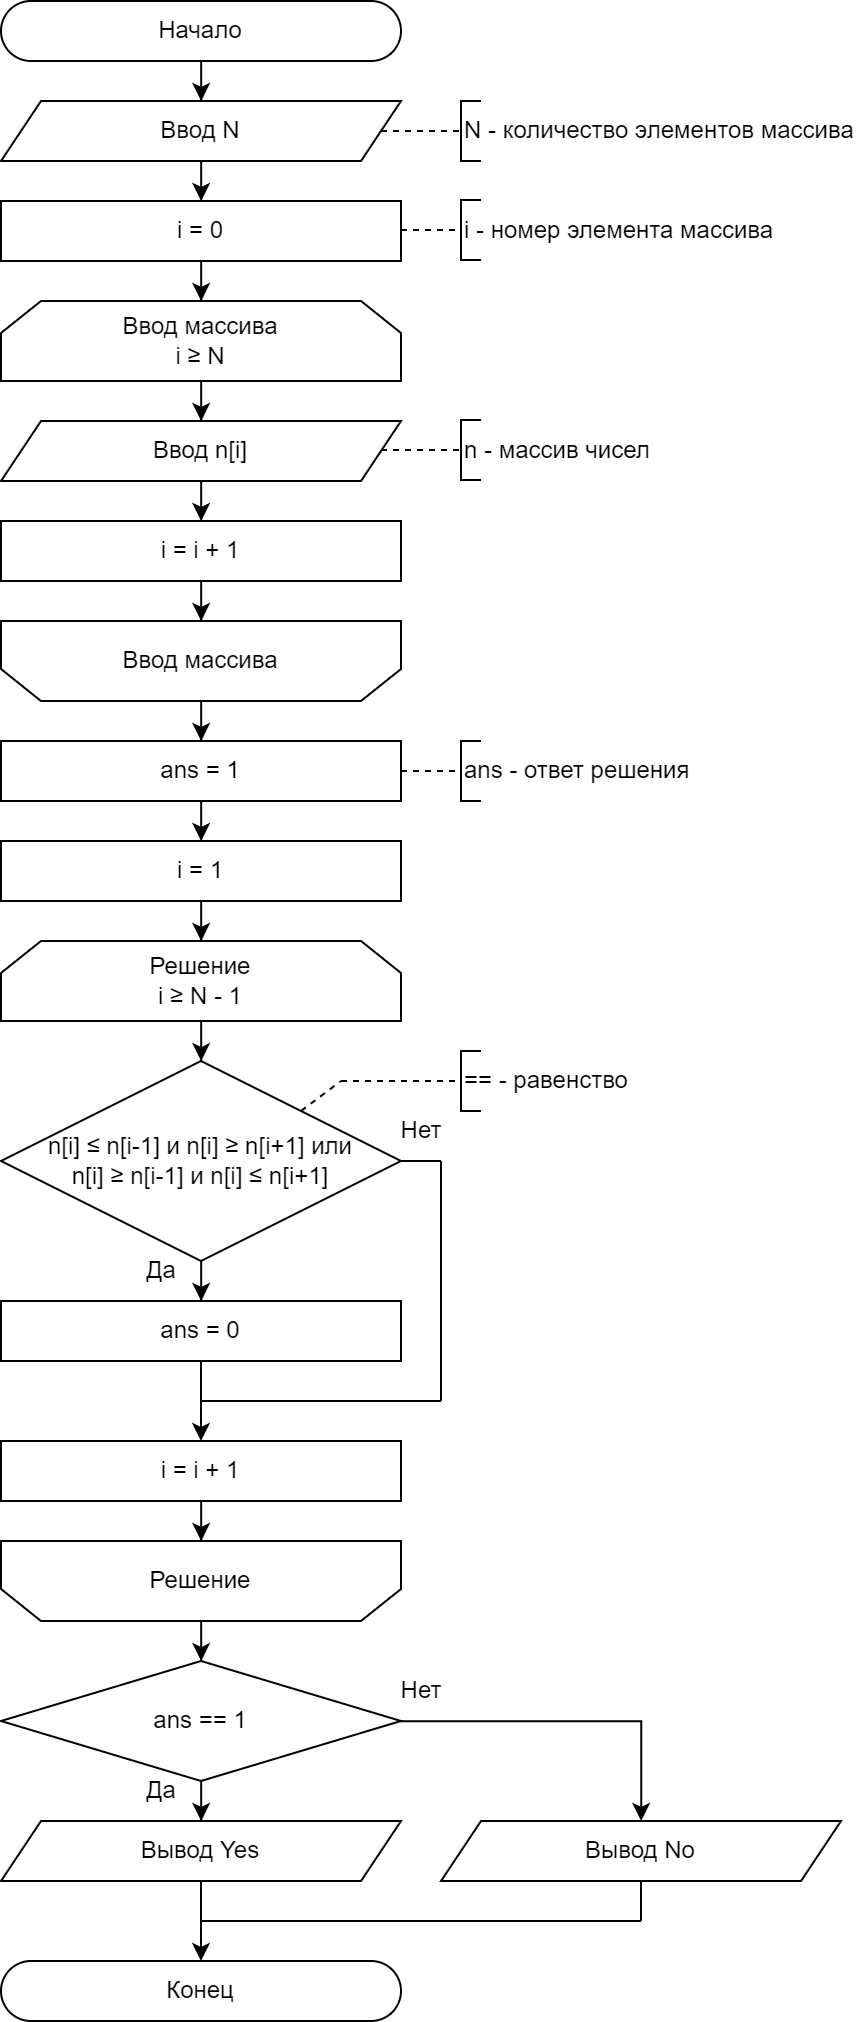
\includegraphics[width=0.49\linewidth]{schemes/s-9}
	\end{figure}
	\begin{center}
		Рисунок 9 – Схема алгоритма задания 9
	\end{center}
	\pagebreak
	\begin{lstlisting}[tabsize=2,basicstyle=\ttfamily]
program solution21;
var N, i, ans:integer;
var a: array[1..64] of integer;
begin
	read(N);
	for i := 1 to N do
		read(a[i]);
	ans := 1;
	for i := 2 to N - 1 do
		begin
		if (a[i] <= a[i - 1]) and (a[i] >= a[i + 1]) or
				(a[i] >= a[i - 1]) and (a[i] <= a[i + 1]) then
			ans := 0;
		end;
	if ans = 1 then
		write('Yes')
	else
		write('No');
end.
	\end{lstlisting}
	
	\newpage
	\subsection*{Задание 10}
	\begin{figure}[h]
		\centering
		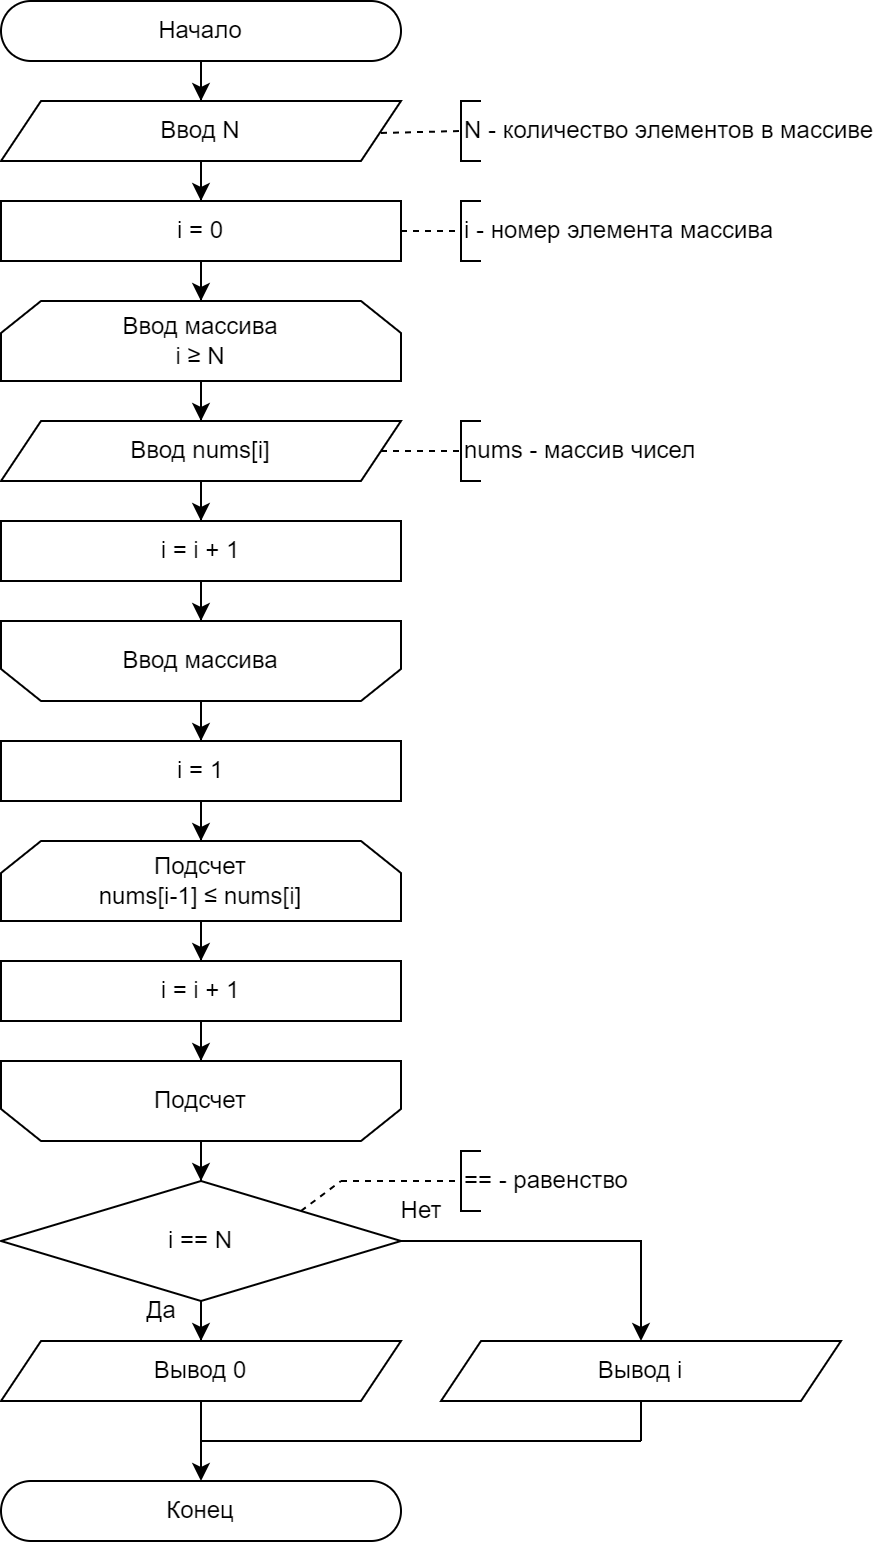
\includegraphics[width=0.6\linewidth]{schemes/s-10}
	\end{figure}
	\begin{center}
		Рисунок 10 – Схема алгоритма задания 10
	\end{center}
	\begin{lstlisting}[tabsize=2,basicstyle=\ttfamily]
#include <stdio.h>
int main() {
	int N;
	scanf("%d", &N);
	float nums[N];
	for (int i = 0; i < N; i++) {
		scanf("%f", &nums[i]);
	}
	int i = 1;
	while (nums[i - 1] <= nums[i]) {
		i++;
	}
	if (i == N) {
		printf("%d", 0);
	} else {
		printf("%d", i);
	}
	return 0;
}
	\end{lstlisting}
	
	\section*{Вывод}
	В ходе выполнения лабораторной работы были решены задачи, которые позволили закрепить и освоить на практике знания о использовании массивов совместно с выполнением арифметических операций, использованием условных конструкций, циклов.
	
\end{document}